\documentclass{templateNote}
\usepackage{tcolorbox}
\usepackage{hyperref}
% \usepackage{pgfplots}
\usepackage{amsmath}
\usepackage{array}
\usepackage{tabularx}
\usepackage{hyperref}
\usepackage{amssymb}

\begin{document}

\imagenlogoU{img/logoNGMFormal_sinF.png}
\linklogoU{https://github.com/NicoGomezM} 
% \imagenlogoD{img/logo-ubb-txt-face.png} 
% \linkQRDoc{https://github.com/NicoxlkboUni} %TODO: Eliminar este qr
\titulo{Unidad 1}
\asignatura{Gestión Estrategica}
\autor{
    \indent
    Nicolás \textsc{Gómez Morgado}
}

\portada
\margenes % Crear márgenes
\tableofcontents
\newpage

\section{Conceptos a tener en cuenta}
\begin{itemize}
    \item Estado $\neq$ Gobierno.
    \item Estado: Conjunto de personas que habitan el país.
    \item Gobierno: Administración del Estado.
    \item Estado de derecho: Las decisiones son tomadas por el congreso. 
    \item \hypertarget{stake}{Stakeholders: Personas que tienen interés en la empresa. (Clientes, proveedores, trabajadores, etc.)}
    \item \hypertarget{sec_ind}{Sector industrial:} Conjunto de empresas que producen bienes o servicios similares.
\end{itemize}
\begin{center}
\begin{tabularx}{\textwidth}{|>{\raggedright\arraybackslash}p{3cm}|X|}
    \hline
    \textbf{Termino} & \textbf{Definición} \\
    \hline
    Misión & Propósito genérico acorde con las necesidades/expectativas de los \hyperlink{stake}{Stakeholders}\\ 
    \hline
    Visión o intención estratégica & Imagen futura de la organización; estado futuro deseado; aspiración de lo que se desea ser (Objetivo a largo plazo) \\
    \hline
    Meta & Afirmación genérica del propósito (afirmar la misión de una forma mas genérica) \\
    \hline
    Objetivo & Cuantificación de la meta (Ej: Aumentar ventas en un 10\%). \\
    \hline
    Núcleo de competencias & Recursos, habilidades y/o procesos que permiten tener una ventaja competitiva. \\
    \hline
    Estrategias & Disección de la forma en que se alcanzaran los objetivos a largo plazo \\
    \hline
    Arquitectura estratégica & Conjunto de los recursos, procesos y competencias para llevar a cabo la estrategia. \\
    \hline
    Control & Controlar las acciones para alcanzar la maxima efectividad de las estrategias. \\
    \hline
\end{tabularx}
\end{center}
\newpage

\section{Tipos de Organizaciones:}
\begin{itemize}
    \item Según lo que produce:
        \begin{itemize}
            \item Primarias
            \item Secundarias
            \item Terciarias
        \end{itemize}
    \item Según actividad desarrollada:
        \begin{itemize}
            \item Agropecuarias
            \item Mineras
            \item Manufactureras
            \item Servicios (Universidades por ejemplo)
        \end{itemize}
    \item Según su fin:
        \begin{itemize}
            \item Con fines de lucro
            \item Sin fines de lucro (Sus fondos se invierten en la organización)
            \begin{itemize}
                \item Fundaciones
                \item Corporaciones
            \end{itemize}
        \end{itemize}
    \item Según tipos de bienes que produce:
        \begin{itemize}
            \item Consumo final
            \item Bienes Intermedios
        \end{itemize}
    \item Según formas de producción:
        \begin{itemize}
            \item Artesanal (Trabajo manual)
            \item Tecnología media
            \item Alta tecnología
        \end{itemize}
    \item Según quien la dirige o decide:
        \begin{itemize}
            \item Autogestiones (Jefe es la autoridad total)
            \item Heterogestionada (Multitud de jefes a través de acciones)
            \item Cogestionada (Decisiones tomadas por jefe y gerente/s)
        \end{itemize}
    \item Según su localización:
        \begin{itemize}
            \item Local (Empresa con ubicación única)
            \item Nacional (Empresa con multiples ubicaciones en el país)
            \item Internacional (Empresa con ubicaciones en varios países)
        \end{itemize}
    \item Según forma de gestión;
        \begin{itemize}
            \item Centralizada (Manejo general)
            \item Descentralizada (Manejo individual por sucursal)
        \end{itemize}
    \item Según propiedad o aportes de capital:
        \begin{itemize}
            \item De personas
                \begin{itemize}
                    \item Responsabilidad limitada
                    \item Responsabilidad ilimitada
                \end{itemize}
            \item De capital
                \begin{itemize}
                    \item Sociedad anónima cerrada
                    \item Sociedad anónima abierta
                \end{itemize}
            \item Mixta o comandita
            \item Cooperativa
            \item Publicas
        \end{itemize}
    \item Según tamaño y estructura:
        \begin{itemize}
            \item Artesanal (1-9 trabajadores)
            \item Pequeña empresa (19-49 trabajadores)
            \item Mediana empresa (50-199 trabajadores)
            \item Gran empresa (200 o más trabajadores)
        \end{itemize}
    \item Según nivel de ventas:
        \begin{itemize}
            \item Microempresa (Hasta 1000 UF)
            \item Pequeña empresa (Hasta 25000 UF)
            \item Mediana empresa (Hasta 100000 UF)
            \item Gran empresa (Más de 100000 UF)
        \end{itemize}
    \item Según estructura:
        \begin{itemize}
            \item Formal (Planificación y estructura jerárquica)
            \item Informal (Nace de forma espontanea por afición de personas e intereses comunes)   
        \end{itemize}
\end{itemize}
\newpage

\section{Administración Estratégica}
\noindent La estrategia de negocios como dirección y alcance de una organización a largo plazo, permite \textbf{obtener ventajas competitivas} en un entorno cambiante, mediante una configuración
    de recursos que permita hacer frente a los mercados y satisfacer las necesidades de los \hyperlink{stake}{\textit{Stakeholders}}.\\

\subsection{Procesos de la Administración Estratégica}
\begin{itemize}
    \item Selección de la misión y objetivos
    \item Análisis del entorno competitivo externo (Oportunidades y Amenazas)       
    \item Análisis del entorno competitivo interno (Fortalezas y Debilidades)
    \item Formulación de estrategias (Decidir el camino de la empresa)
    \item Implementación de estrategias (Como y quien hace las cosas)
    \item Control de estrategia (Chequeo antes, durante y después del proceso)
\end{itemize}

\subsection{Triangulo de la administración estratégica.}
\begin{figure}[H]
    \centering
    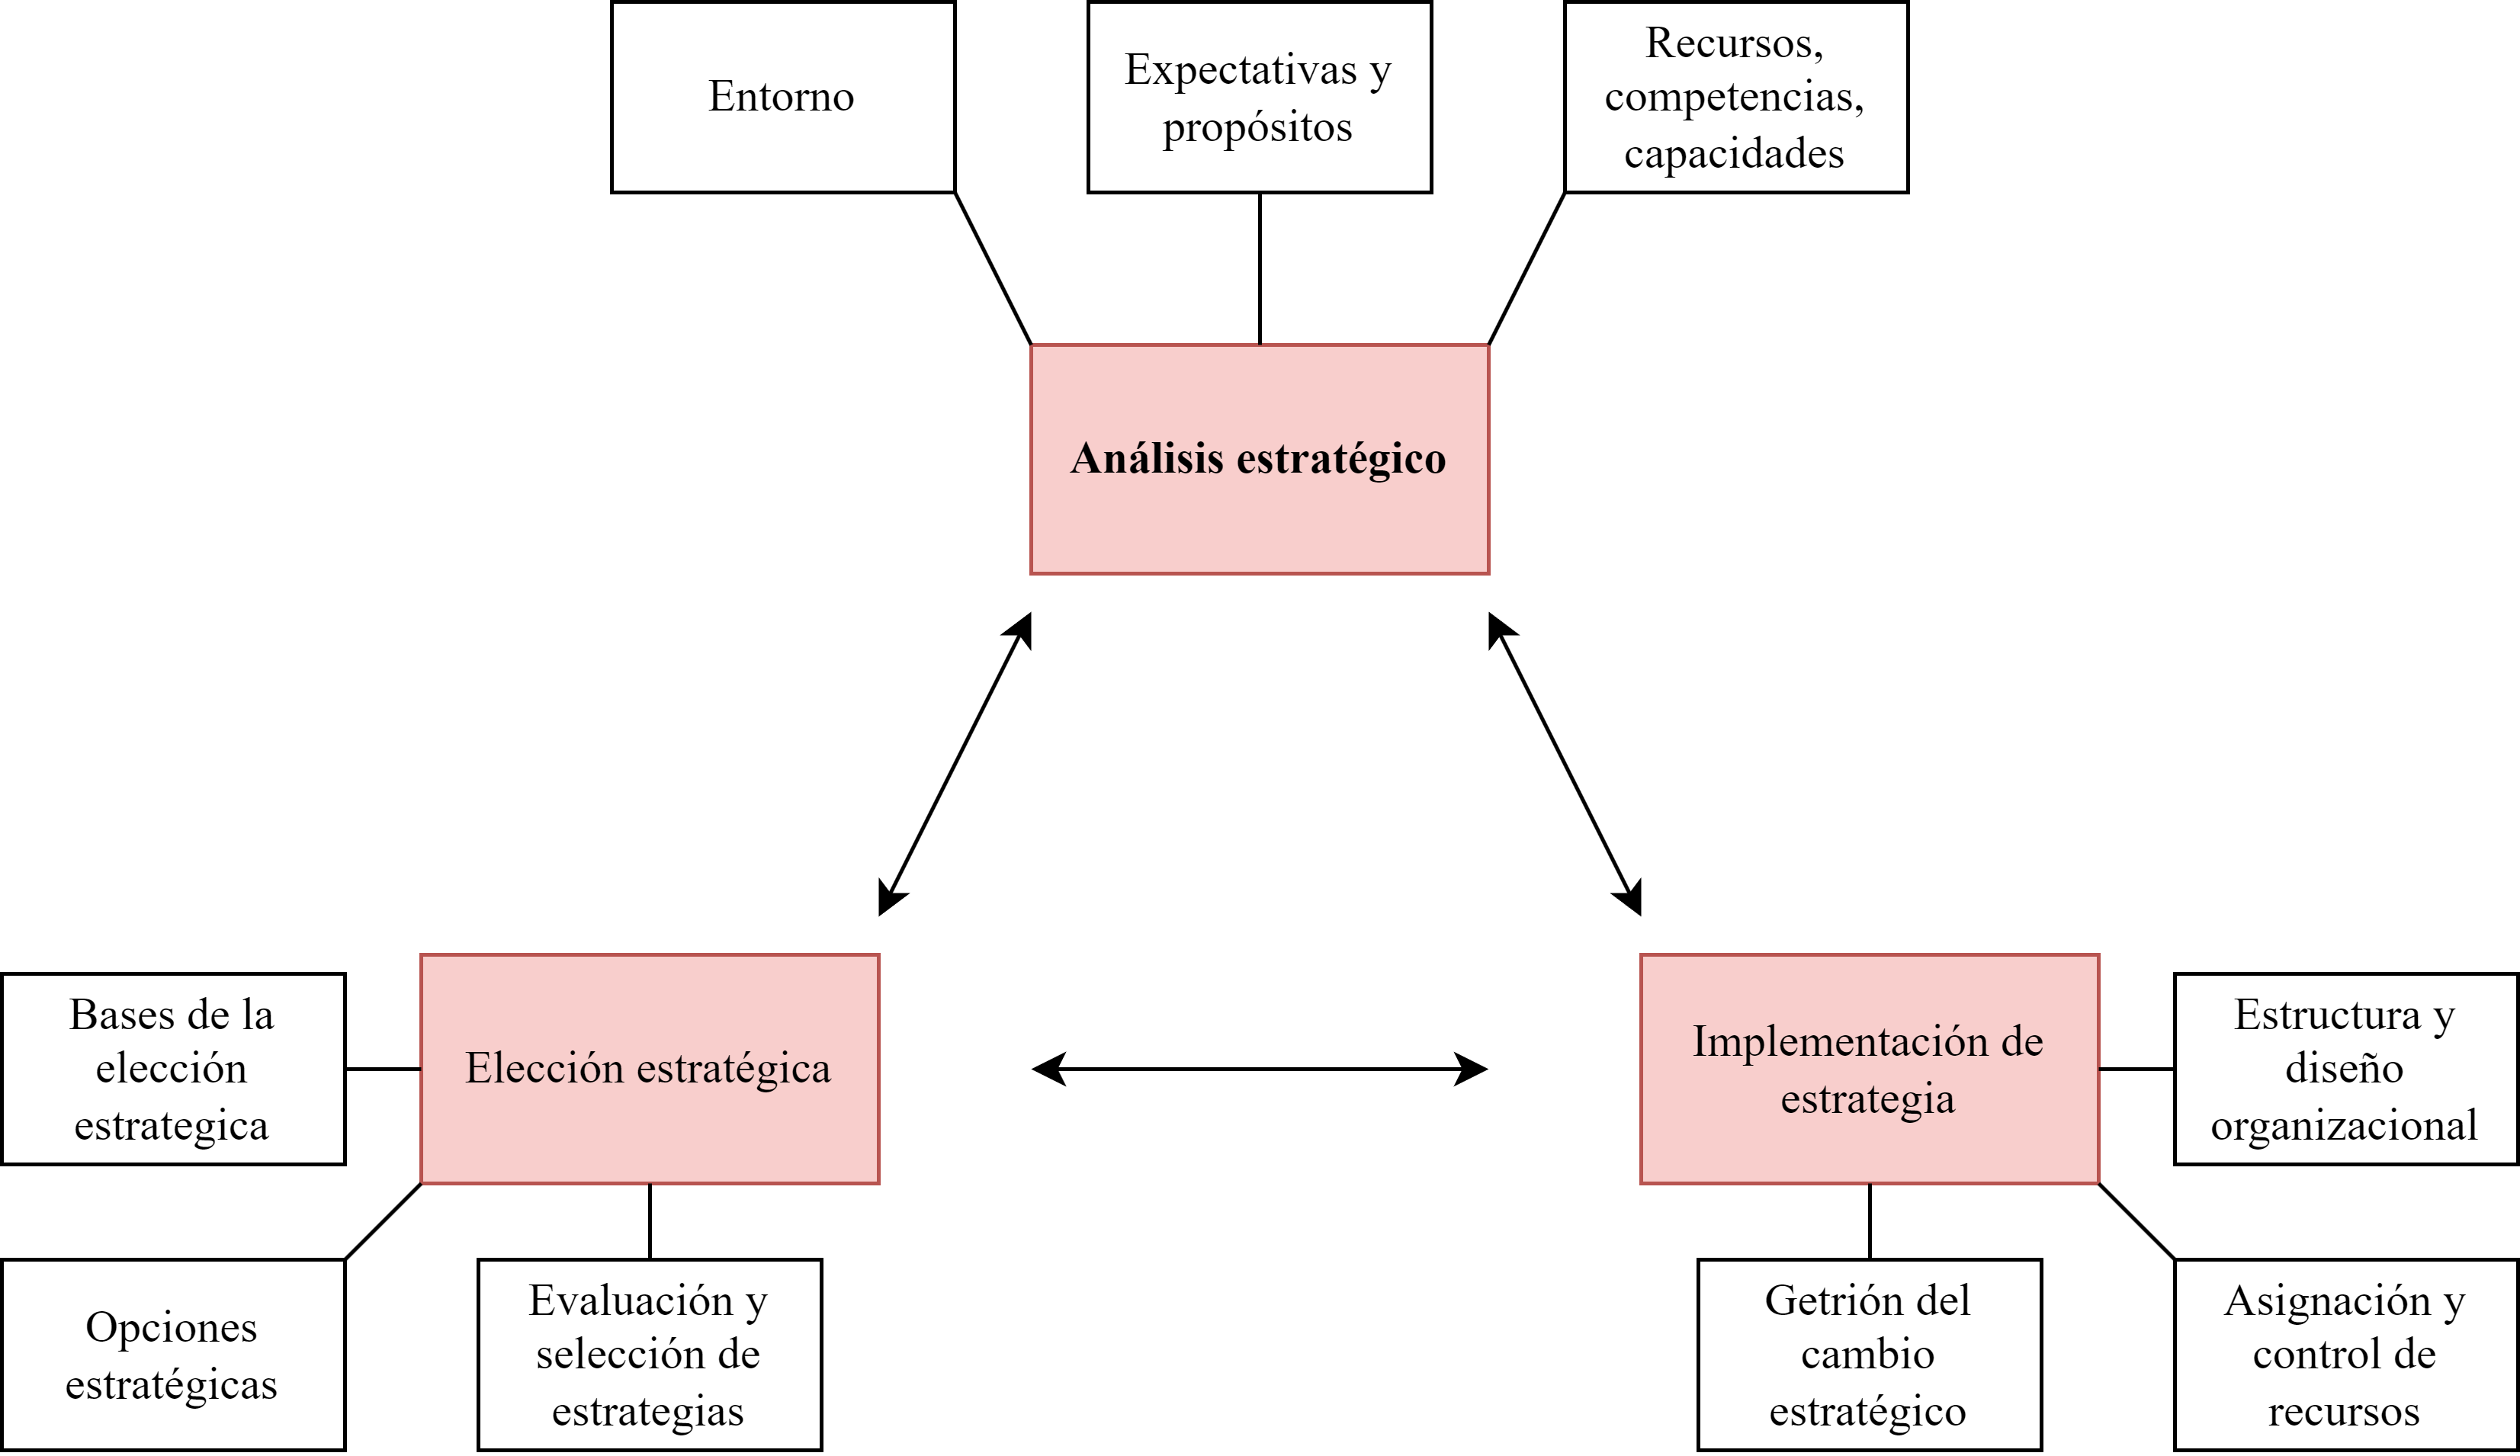
\includegraphics[width=0.8\textwidth]{img/triangulo.png}
\end{figure}
\newpage


\section{Análisis estratégico}
\begin{itemize}
    \item \textbf{El entorno:} Conjunto de factores que rodean a la empresa y que influyen en su funcionamiento.
    \item \textbf{Expectativas y propósitos:} Objetivos que se desean alcanzar.
    \item \textbf{Recursos:} Elementos que se utilizan para alcanzar los objetivos.
    \item \textbf{Competencias:} Habilidades y destrezas que permiten alcanzar los objetivos.
    \item \textbf{Capacidades:} Conjunto de recursos y competencias que permiten alcanzar los objetivos.
\end{itemize}

\subsection{Entorno}
\noindent Tanto el entorno empresarial como el económico global se ven afectados por distintos factores frente a los cuales estos entes 
    deben enfrentarse a la \textbf{necesidad de una reconsideración} de sus estrategias. Algunos de estos factores son:\\

\begin{itemize}
    \item Liberalización: Reducción de restricciones comerciales de parte del gobierno lo cual facilita el libre comercio y la inversion.
    \item Cambios estructurales: Cambios duraderos y significativos en la estructura de la economía, como la globalización.
    \item Competencia global: Competencia entre empresas de distintos países.
    \item Bloques de comercio: Agrupaciones de países que establecen acuerdos comerciales.
    \item Discontinuidad tecnológica: Cambios tecnológicos que afectan la forma de hacer negocios.
    \item Exceso de capacidad: Producción de bienes o servicios en exceso.
    \item Fusiones y adquisiciones: Compra de una empresa por otra.
    \item Preocupación medioambiental: Preocupación por el impacto ambiental de las empresas.
    \item Expectativas cambiantes de los clientes: Cambios en las preferencias de los consumidores.
    \item Menor proteccionismo: Menos políticas proteccionistas por parte de los gobiernos, lo que promueve un mercado más abierto y competitivo.
\end{itemize}

\subsubsection{Exploración ambiental de la organizacion}
\noindent La exploración ambiental de la organización es un proceso que permite identificar y analizar los factores del entorno que pueden afectar a la empresa. 
    Este proceso se lleva a cabo a través de la recolección de información y el análisis de los datos obtenidos. Algunos de los ambientes \textbf{críticos} existentes son:

    \begin{itemize}
        \item \textbf{Ambiente de clientes:} Comprender y analizar las características y comportamientos de los clientes actuales y potenciales, incluyendo variables demográficas, y mantener comunicación e intercambio de información para ganar su confianza y establecer relaciones comerciales.
        \item \textbf{Ambiente competidores:} Analizar la identidad, motivos, fortalezas, debilidades y conductas de las empresas competidoras, así como sus métodos para llegar a los clientes deseados. Incluso sus clientes pueden volverse competidores (Modelo de Rivalidad Ampliada).
        \item \textbf{Cambio de proveedores:} Los cambios de proveedores impactan los costos de inversión, precios, demanda, márgenes de contribución, suministros, procesos de producción, requisitos de inversión, costos y disponibilidad.
        \item \textbf{Ambiente competitivo:} El ambiente competitivo influye en la adopción de nuevas tecnologías, afectando costos y calidad de productos; la entrada de nuevos competidores impacta precios, participación de mercado y márgenes de contribución; y el lanzamiento de nuevos productos modifica la demanda y los gastos en publicidad.
        \item \textbf{Cambios en el mercado:} Los cambios en el mercado incluyen nuevos usos de productos que afectan la demanda y utilización de capacidades, nuevos mercados que influyen en los canales de distribución, demanda y uso de capacidades, y la obsolescencia de productos que impacta precios, demanda y utilización de capacidades.
        \item \textbf{Ambiente económico:} El ambiente económico se ve afectado por las tasas de interés, las tasas de cambio y los cambios en el ingreso per cápita, los cuales influyen en la expansión económica, la demanda interna y externa, así como en los beneficios empresariales.
        \item \textbf{Ambiente tecnológico:} El ambiente tecnológico influye en los costos y la calidad de los productos, la aparición de nuevos competidores, la determinación de precios, el desarrollo de nuevos productos, los cambios en los canales de distribución, la demanda y la utilización de capacidades, así como en la obsolescencia de productos.
        \item \textbf{Ambiente social:} Los cambios en las preferencias de los clientes y las tendencias demográficas afectan la demanda y el diseño de productos, mientras que la incorporación al mercado laboral influye en los costos. La profesionalización del personal incide en los costos y la productividad, y la globalización impacta en los costos, la demanda y la competitividad.
        \item \textbf{Ambiente politico:} Los cambios en la legislación y regulación afectan los costos, la demanda y la competitividad, mientras que la estabilidad política influye en la inversión y la demanda.
        \item \textbf{Ambiente legal:} Los cambios en la legislación y regulación afectan los costos, la demanda y la competitividad, mientras que la estabilidad política influye en la inversión y la demanda.
        \item \textbf{Ambiente físico:} Los cambios en el ambiente físico afectan la demanda y la utilización de capacidades, mientras que la disponibilidad de recursos naturales influye en los costos y la competitividad.
    
    \end{itemize}


\subsection{Estrategia competitiva}
\noindent Búsqueda de posición favorable en uno o mas sectores del mercado; Las ventajas competitivas de una empresa se basan principalmente en la capacidad de la empresa para ofrecer un valor único y significativo a sus clientes. \\
Inciden en la elección de la estrategia competitiva:
\begin{itemize}
    \item \textbf{Atractivo del sector} para obtener utilidades a largo plazo y los factores determinantes.
    \item Determinantes de una \textbf{posición competitiva} relativa dentro de un sector especifico.
    \item Ambos factores anteriores son dinámicos y cambian con el tiempo.
\end{itemize}

\subsection{Modelos estratégicos basados en el sector industrial}

\subsubsection{Modelo competitivo (Atractivo del sector)}
\noindent Se basa en las fuerzas que mueven a la competencia en un \hyperlink{sec_ind}{sector industrial}, las cuales determinan la rentabilidad a largo plazo de las empresas en dicho sector.\\

\noindent\underline{\textbf{Fuerzas que mueven a la competencia}}\\\\
- La rivalidad ampliada determina el grado de la competencia dentro de la industria.\\
- El éxito de una empresa en un \hyperlink{sec_ind}{sector industrial} dependerá de su propia estrategia. \\
- EL estudio del modelo Porter permite:
\begin{itemize}
    \item Definir una estrategia competitiva mas ad-hoc.
    \item Buscar una posición del sector donde la empresa pueda defenderse de las 5 fuerzas o usarlas a su favor.
\end{itemize} 
\textbf{Las 5 fuerzas de Porter}
    \begin{itemize}
        \item Amenaza ingreso de nuevos competidores potenciales (ANE)
        \begin{itemize}
            \item Características:
            \begin{itemize}
                \item Aporta capacidad adicional.
                \item Nuevo competidor altera participación del mercado.
            \end{itemize}
            \item Consecuencias:
            \begin{itemize}
                \item Disminución de precios.
                \item Aumento de costos.
                \item Reducción rentabilidad.
            \end{itemize}
        \end{itemize}
        \item Amenaza de productos sustitutos (APS)
        \begin{itemize}
            \item Características:
            \begin{itemize}
                \item Producto sustituto reemplaza a otro.
                \item Producto sustituto reduce rentabilidad.
            \end{itemize}
            \item Consecuencias:
            \begin{itemize}
                \item Si el precio de los productos es alto, los \\clientes optaran por el producto sustituto.
            \end{itemize}
        \end{itemize}
        \item Rivalidad competidores existentes (RC)
        \begin{itemize}
            \item Características:
            \begin{itemize}
                \item Surge presión u oportunidad para mejorar posición.
            \end{itemize}
            \item Consecuencias:
            \begin{itemize}
                \item Aumento competencia via precios.
                \item Batallas publicitarias.
            \end{itemize}
        \end{itemize}
        \item Poder negociador de los clientes (PNC)
        \begin{itemize}
            \item Características:
            \begin{itemize}
                \item Clientes pueden forzar reducción de precios.
                \item Exigencia por mayor calidad de productos/servicios.
            \end{itemize}
            \item Consecuencias:
            \begin{itemize}
                \item Aumento competencia entre competidores.
            \end{itemize}
        \end{itemize}
        \item Poder negociador de los proveedores (PNP)
        \begin{itemize}
            \item Características:
            \begin{itemize}
                \item Proveedores pueden forzar aumento de precios.
                \item Proveedores pueden reducir calidad de productos/servicios.
                \item Asociación proveedores fuera de la industria.
            \end{itemize}
            \item Consecuencias:
            \begin{itemize}
                \item Fijación precio y calidad de insumos adquiridos por la industria.
            \end{itemize}
        \end{itemize}
\end{itemize}

\subsubsection{Porfolio de mercado (BCG)}


\subsection{Elementos que dan valor a la estrategia}
\begin{itemize}
    \item Recursos limitados.
    \item Comportamiento competidor.
    \item Compromiso irreversible recursos.
    \item Necesidad coordinación acciones a distancia en el tiempo.
    \item Incertidumbre acerca control de iniciativa.
    \item Percepciones reciprocas entre adversarios.
\end{itemize}

\subsection{Requisitos para el desarrollo de una estrategia}
\begin{itemize}
    \item Conocimientos.
    \item Capacidad para la integración.
    \item Pericia en el análisis de sistemas para comprender racionalidad, periodicidad, posibilidades y consecuencias inmediatas/futuras.
    \item Imaginación y lógica para elegir entre alternativas.
    \item Control de recursos mas allá de la necesidad inmediata.
    \item Capacidad de renunciar a beneficios inmediatos por beneficios futuros.
\end{itemize}

\subsection{Herramientas para el desarrollo de estrategias}

\subsubsection{Análisis competitivo}
    \begin{itemize}
        \item \textbf{Análisis FODA}
        \begin{itemize}
            \item \textbf{Fortalezas:} Ventajas con respecto a otras empresas las cuales mejoro o potencio.
            \item \textbf{Oportunidades:} Situaciones que ofrece el entorno en las cuales la empresa puede obtener algún tipo de beneficio.
            \item \textbf{Debilidades:} Implican costos o resultados negativos en su entorno, se buscan minimizar o eliminar.
            \item \textbf{Amenazas:} Situaciones presentes en el entorno que pueden afectar negativamente a la empresa, ante las cuales se prevenga o prepare.
        \end{itemize}
    \end{itemize}

\subsubsection{Análisis de cartera de actividades}
    \begin{itemize}
        \item \textbf{Matriz BCG} (Boston Consulting Group)
        \begin{itemize}
            \item \textbf{Estrellas:} Productos con alta participación en el mercado y alto crecimiento. \textbf{(Relevar a las vacas lecheras)}
            \item \textbf{Interrogantes:} Productos con baja participación en el mercado y alto crecimiento. \textbf{(Desarrollarse o retirarse)}
            \item \textbf{Vacas lecheras:} Productos con alta participación en el mercado y bajo crecimiento. \textbf{(Cosechar utilidades)}
            \item \textbf{Perros:} Productos con baja participación en el mercado y bajo crecimiento. \textbf{(Retirarse o sobrevivir)}
        \end{itemize}
        \begin{figure}[H]
            \centering
            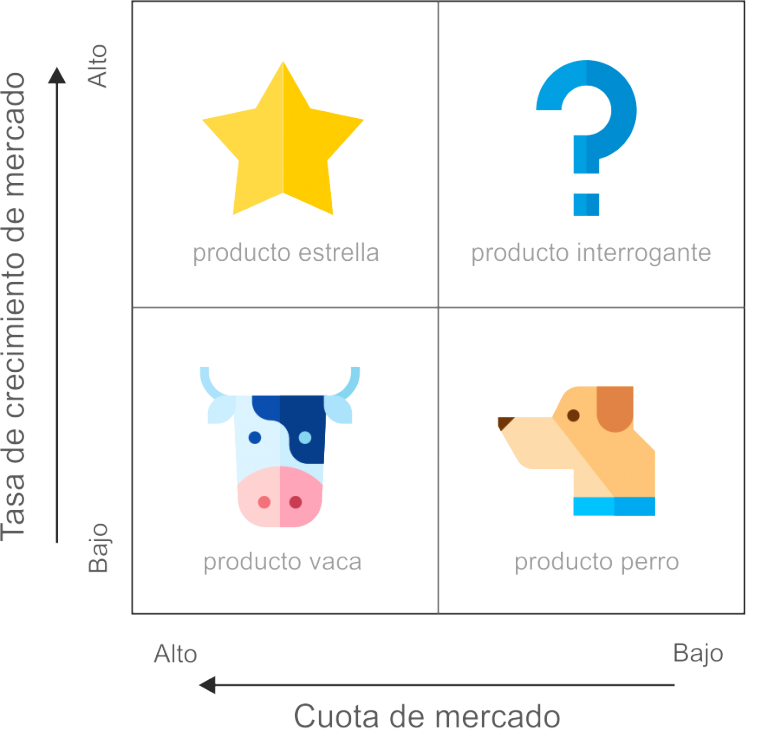
\includegraphics[width=0.5\textwidth]{img/matriz_bcg-768x803.png}
        \end{figure}
        \item \textbf{Matrices de Planificación}
        \begin{itemize}
            \item \textbf{Matriz de crecimiento-participación:} Analizar como funcionaria nuestra empresa en el mercado.
            \begin{itemize}
                \item Factores externos: Crecimiento del mercado.
                \item Factores internos: Participación relativa en el mercado.
            \end{itemize}
            \item \textbf{Matriz atractivo de la industria-fortaleza del negocio:} Analizar la industria, ver competencia y ventaja competitiva.
            \begin{itemize}
                \item Factores externos: Atractivo de la industria.
                \item Factores internos: Fuentes de ventaja competitiva.
            \end{itemize}
            \begin{figure}[H]
                \centering
                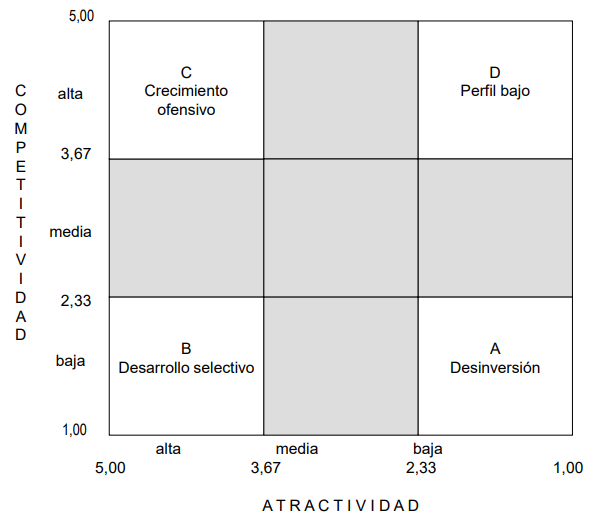
\includegraphics[width=0.4\textwidth]{img/matriz_atractivo.png}
            \end{figure}
            \item \textbf{Matriz Ciclo de vida:} Analizar el tiempo de respuesta del consumidor con respecto a un producto o servicio.
            \begin{itemize}
                \item Factores externos: Madurez de la industria.
                \item Factores internos: Medición general de la posición del negocio.
            \end{itemize}
            \item \textbf{Matriz tamaño ventaja competitiva:} Análisis especifico de nuestra ventaja con respecto a otras empresas.
            \begin{itemize}
                \item Factores externos: Formas de competir (oportunidades de diversificación).
                \item Factores internos: Tamaño/sostenibilidad de la/s ventaja/s competitiva/s.
            \end{itemize}
            \item \textbf{Matriz rentabilidad:} Comparación entre la inversion y la utilidad. 
            \begin{itemize}
                \item Factores externos: Potencial del crecimiento del mercado; Costo de capital.
                \item Factores internos: Rentabilidad; Generación de fondos.
            \end{itemize}
        \end{itemize}
    \end{itemize}

\subsubsection{Análisis de la cadena de valor}
\begin{itemize}
    \item \textbf{Ciclo de vida}
    \begin{itemize}
        \item \textbf{Introducción:} Producto entrando en el mercado.
        \item \textbf{Aceptación:} Producto comienza a ser aceptado por el mercado objetivo.
        \item \textbf{Madurez:} Producto se estabiliza en el mercado y alcanza su punto máximo de ventas.
        \item \textbf{Saturación:} Producto comienza a perder ventas.
        \item \textbf{Obsolescencia:} Producto deja de ser vendido o el nivel de ventas llega al mínimo (Productos Perros).
    \end{itemize}
\end{itemize}

\subsubsection{Elección de estrategia}
\noindent Para elegir la estrategia a implementar, es imprescindible haber realizado previamente alguno de los análisis mencionados. Una vez completados estos análisis, las estrategias disponibles son:
\begin{itemize}
    \item Estrategia competitiva (genérica)
    \item Estrategia de crecimiento (Dinero) 
    \item Estrategia de desarrollo (Calidad de vida/productos)
\end{itemize}

\subsection{Negocios}
\subsubsection{Categoría de negocios}
\begin{itemize}
    \item \textbf{Volumen:} Alcanzar el punto preciso del mínimo costo y liderar en ventas.
    \item \textbf{Especialización:} Centrarse en un punto del mercado y ser el mejor en ese punto o cubrir todo el mercado con productos con características únicas.
    \item \textbf{Fragmentada:} Llevar a cabo varias formas de competencias, teniendo en cuenta fuerzas relativas y competencias únicas.
    \item \textbf{Estancamiento:} Sobrevivir en el mercado a través de la reducción de costos y maximización de la productividad
\end{itemize}

\subsubsection{Lógica de negocios}
\begin{itemize}
    \item \textbf{Lógica del cliente:} Como tener acceso a los clientes.
    \item \textbf{Lógica del producto:} Oferta diferenciada que se lleva al mercado.
    \item \textbf{Lógica económica:} Obtención de beneficios o satisfacer los criterios establecidos de beneficio económico.
    \item \textbf{Lógica estructural:} Organización necesaria para que las 3 lógicas anteriores operen en conjunto.
\end{itemize}

\begin{figure}[H]
    \centering
    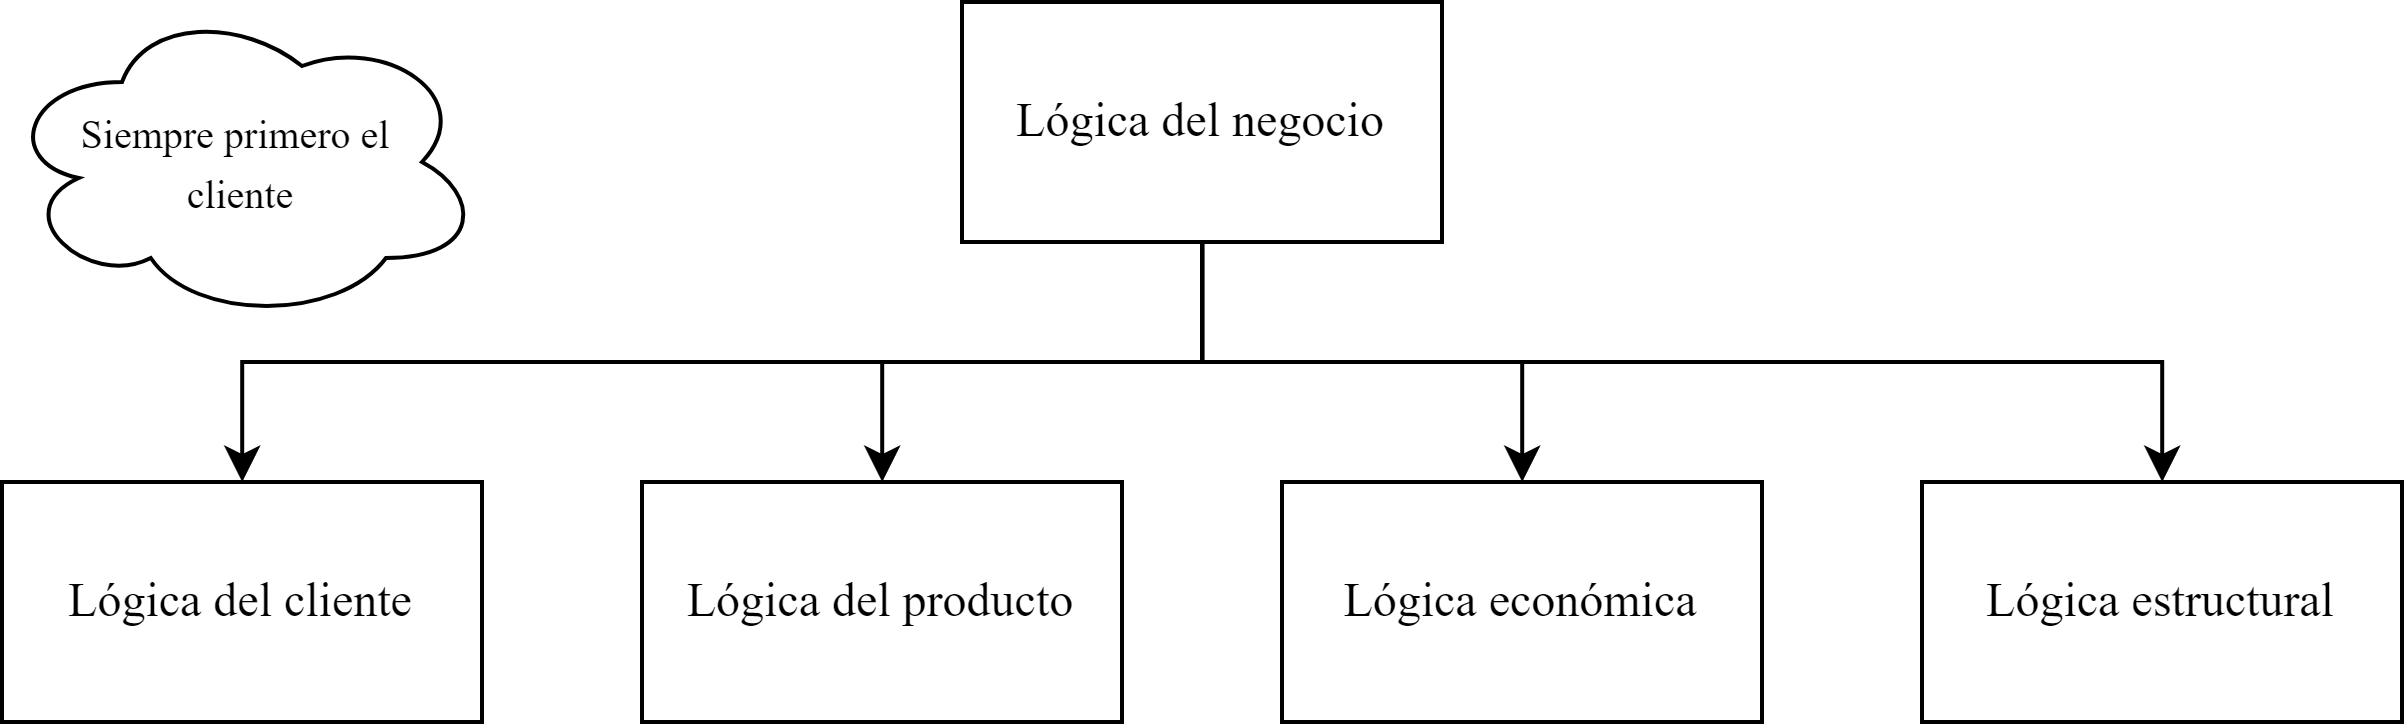
\includegraphics[width=1\textwidth]{img/logicanegocio.png}
\end{figure}

\begin{figure}[H]
    \centering
    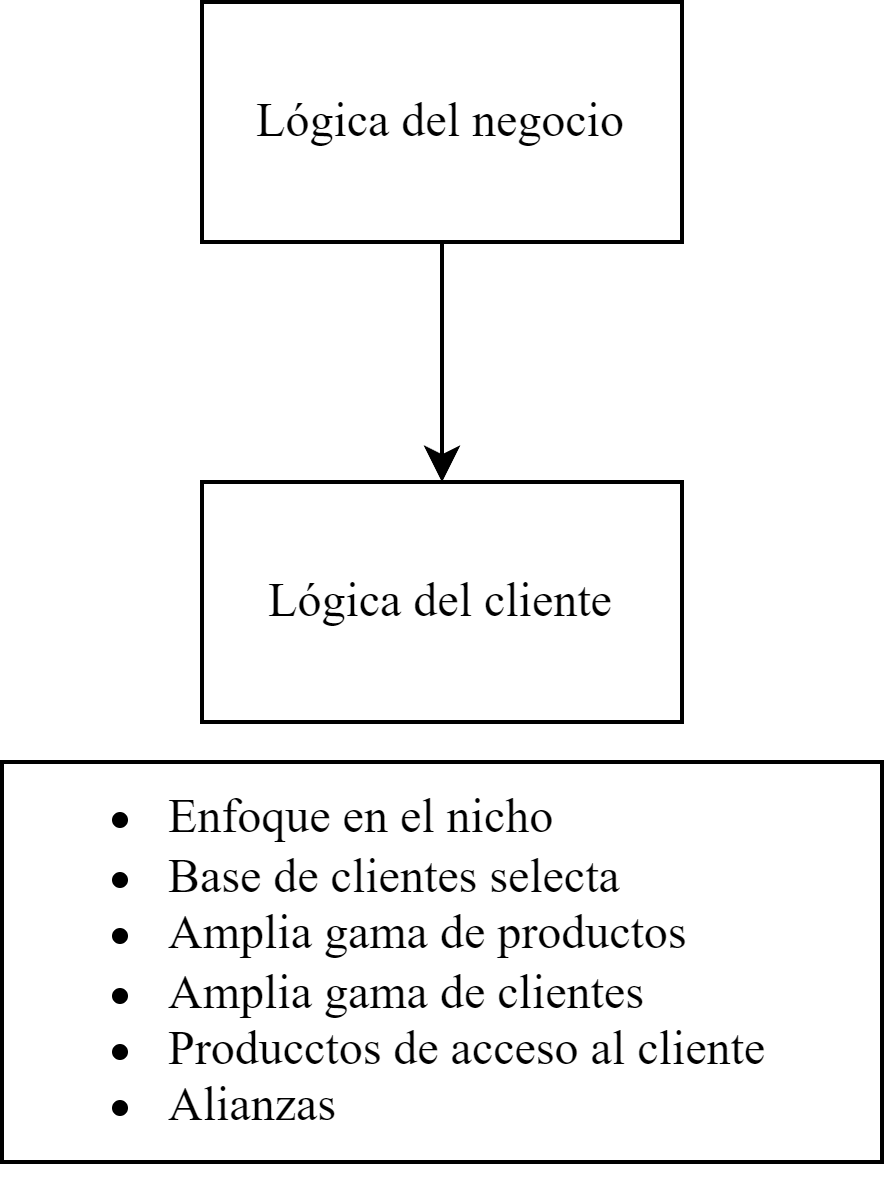
\includegraphics[width=0.45\textwidth]{img/logicacliente.png}
\end{figure}

\subsubsection{Cadena de valor de negocios}
\begin{figure}[H]
    \centering
    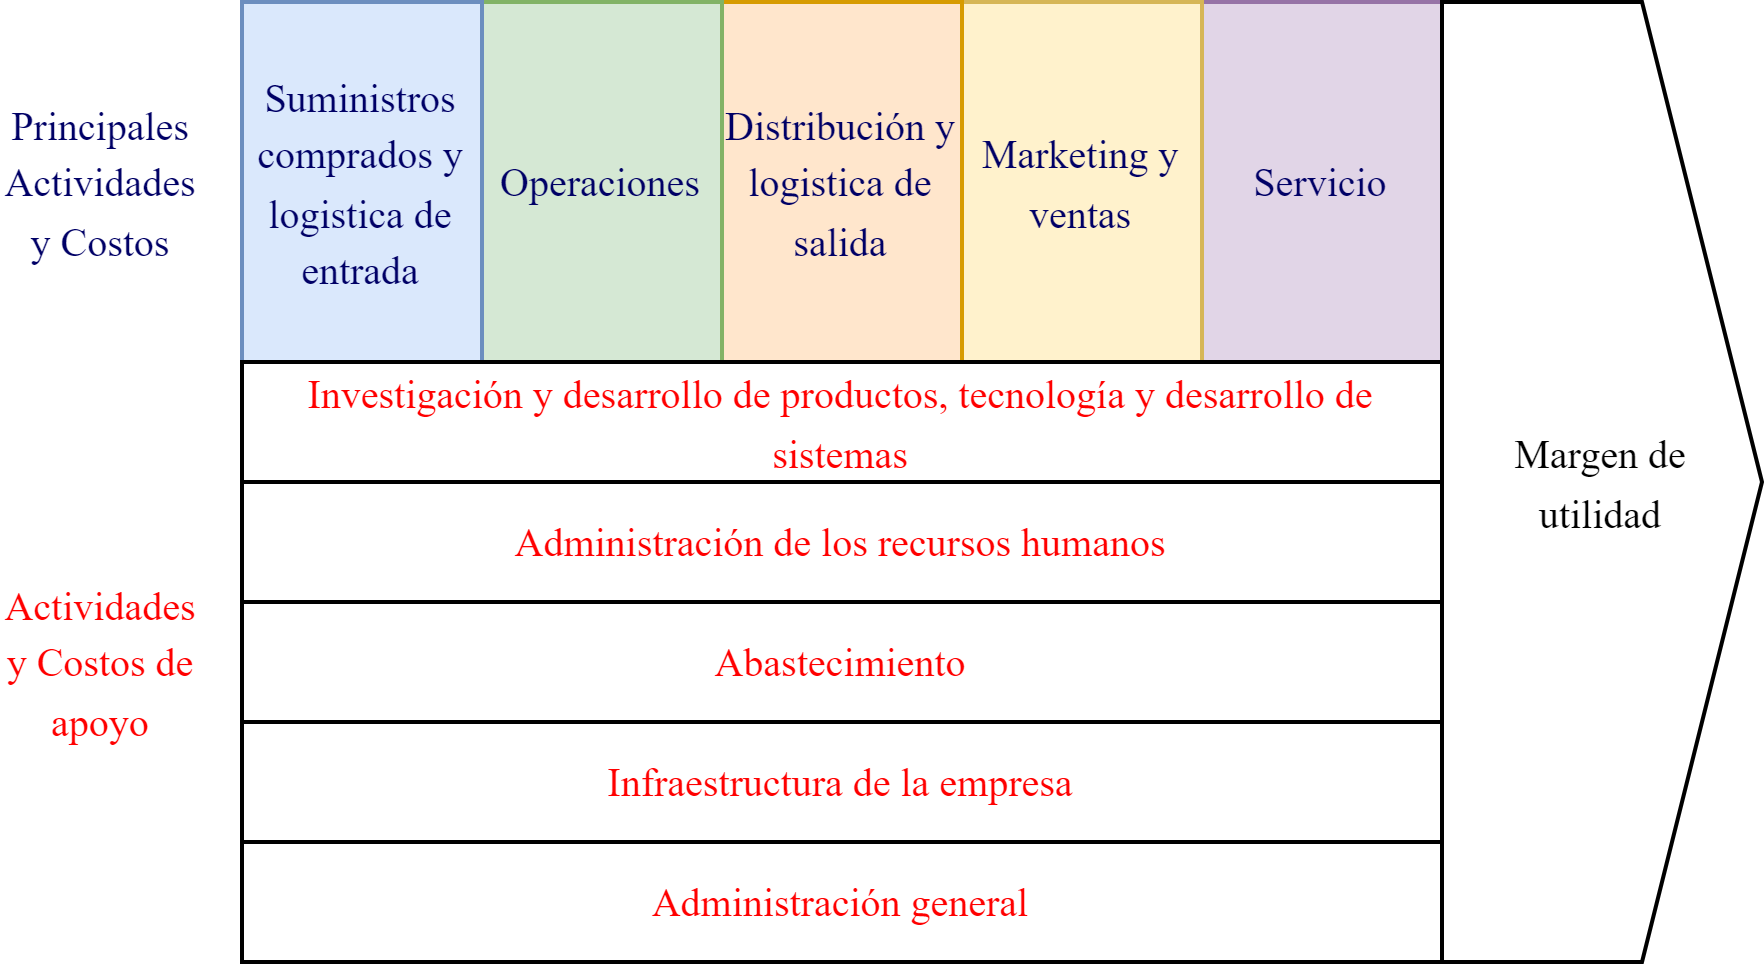
\includegraphics[width=1\textwidth]{img/costosdenoseque.png}
\end{figure}

\begin{itemize}
    \item El desglosar en este diagrama las operaciones de las actividades y procesos nos expone en gran medida los elementos que significan un costo para la empresa.
    \item Todas las actividades en la cadena de valor involucran un costo y limita activos.
    \item El asignar los costos de operación y activos a cada actividad nos permite ver un aproximado del costo respectivo.
    \item La cadena de valor y como se desempeñan las actividades reflejan la evolución del negocio, operaciones internas, estrategias, enfoques de ejecución y las economías de las actividades
\end{itemize}

\newpage


\section{Elección estratégica}
\subsection{Modelo de negocios}
\noindent Enfoque mas estrecho que la estrategia de negocios, esta vinculada con las iniciativa competitivas de la empresa y con los enfoques de negocios.\\\\
El modelo de negocios tiene que ver con que los ingresos y costos asociados a la estrategia demuestran viabilidad de los negocios.\\\\
- Las empresas con mas tiempo en los negocios con generación de utilidades tienen un modelo de negocios probado. Existe evidencia que su estrategia ha sido benéfica y que la empresa es viable\\
- Las empresas con perdida de dinero o en iniciación de actividades siguen un modelo de negocio errado o aun no probado. No se ha demostrado que sus estrategias produzcan buenos resultados y sean viables.

\subsection{Proceso de formulación de estrategias}
\begin{enumerate}
    \item Identificar el proceso o elemento al que se le confeccionara una estrategia.
    \item Análisis FODA del proceso o elemento elegido.
    \item Identificar factores relevantes del proceso escogido.
    \item Decidir si utilizar:
    \begin{enumerate}
        \item 1 variable representativa.
        \item 2 o mas variables representativas.
    \end{enumerate}
    \item Definir resultados esperados de cada estrategia.
    \item Seleccionar estrategia/s mas viable/s.
    \item Elegir estrategia según objetivos planteados.
\end{enumerate}

\subsection{Estrategias}
\hypertarget{estrategia_corporativa}{\noindent\textbf{Nivel 1: \textit{Estrategias corporativas}}}
\indent Misión, vision, definición del negocio.
\begin{itemize}
    \item Liderazgo en costos.
    \item Diferenciación.
    \item Concentración.
\end{itemize}
\textbf{Nivel 2: \textit{Estrategias de cartera (productos - mercado)}}
\textbf{Nivel 3: \textit{Estrategias de segmentación y posicionamiento}}
\textbf{Nivel 4: \textit{Estrategias de funcionales}}

\subsubsection{Estrategias competitivas}
\noindent Dependiendo de la cuota de mercado que posea la empresa:
\begin{itemize}
    \item Estrategias de líder.
    \item Estrategias de retador.
    \item Estrategias de seguidor.
    \item Estrategias de especialista.
\end{itemize}

\subsubsection{Características de las empresas rentables}
\begin{itemize}
    \item Segmentar creativamente.
    \item Utilizar eficazmente variables investigación y desarrollo para disminuir costos y aumentar rentabilidad.
    \item Pensar en pequeño, conforme con su tamaño, poner acento en rentabilidad aprovechando su ventaja competitiva defendible.
    \item Fuerza del directivo que lo lleva a estar implicado, no sólo en la estrategia, sino también en la táctica.
\end{itemize}

\subsubsection{Estrategia corporativa}
\noindent Como se discute en el \hyperlink{estrategia_corporativa}{Nivel 1}, la estrategia corporativa es la que establece el proposito y alcance de la empresa.\\
Su definición incluye dos decisiones trascendentes:
\begin{itemize}
    \item \textbf{Misión de la empresa}.
    \item \textbf{Definición del negocio.}
\end{itemize}
- Define las actividades en las que busca participar y su combinación mas adecuada.\\
- Busca sinergia entre la integración y complementariedad de las actividades de la cartera de negocio.\\

\end{document}
